\subsection{Implementation}
Isolation Forest algorithm is built on the basis of the following assumptions:
\begin{itemize}
    \item \textbf{Fewness} - anomalous samples are rare, constituting only a minority, and they appear in limited numbers within any dataset.
    \item \textbf{Different} - anomalous samples exhibit values or attributes that significantly diverge from those of normal samples.
\end{itemize}

\begin{figure}[H]
  \centering
  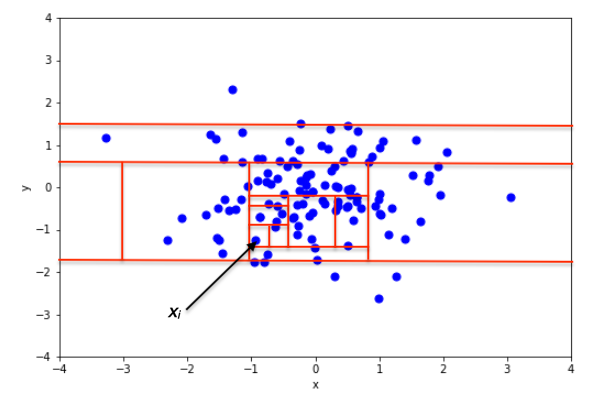
\includegraphics[width=\linewidth]{body/02_methodology/img/figure5.png}
  \caption{Two above assumptions make detecting and isolating anomalous from dataset easier.}
\end{figure}


There are a several python libraries such as ScikitLearn.IsolationForest, which provides a simple and efficient way to implement the algorithm
In submitted code, I used library to implement Isolation Forest algorithm. The library is called \textbf{scikit-learn}. The library provides a simple and efficient way to implement Isolation Forest algorithm. However, to better understand the algorithm, I will try to explain the algorithm in my own words. 

\newpage
Given a dataset $X$ with $n$ samples, the algorithm works as follows:

\begin{enumerate}
    \item Randomly select a feature $f$ from the dataset $X$.
    \item Randomly select a split value $s$ between the maximum and minimum values of feature $f$.
    \item Split the data into two parts: one with values $<= s$ and the other with values $> s$.
    \item Repeat steps 1-3 until either the samples are completely isolated or all the values at the current node are identical.
\end{enumerate}

The algorithm iterates through steps 1-4 several times, generating multiple Isolation Trees, which collectively form an Isolation Forest. By observing how Isolation Trees are constructed and understanding the characteristics of anomalous points, it becomes apparent that the majority of anomalies tend to be positioned closer to the tree's root. This is because they are easier to isolate compared to normal points.

\begin{figure}[H]
  \centering
  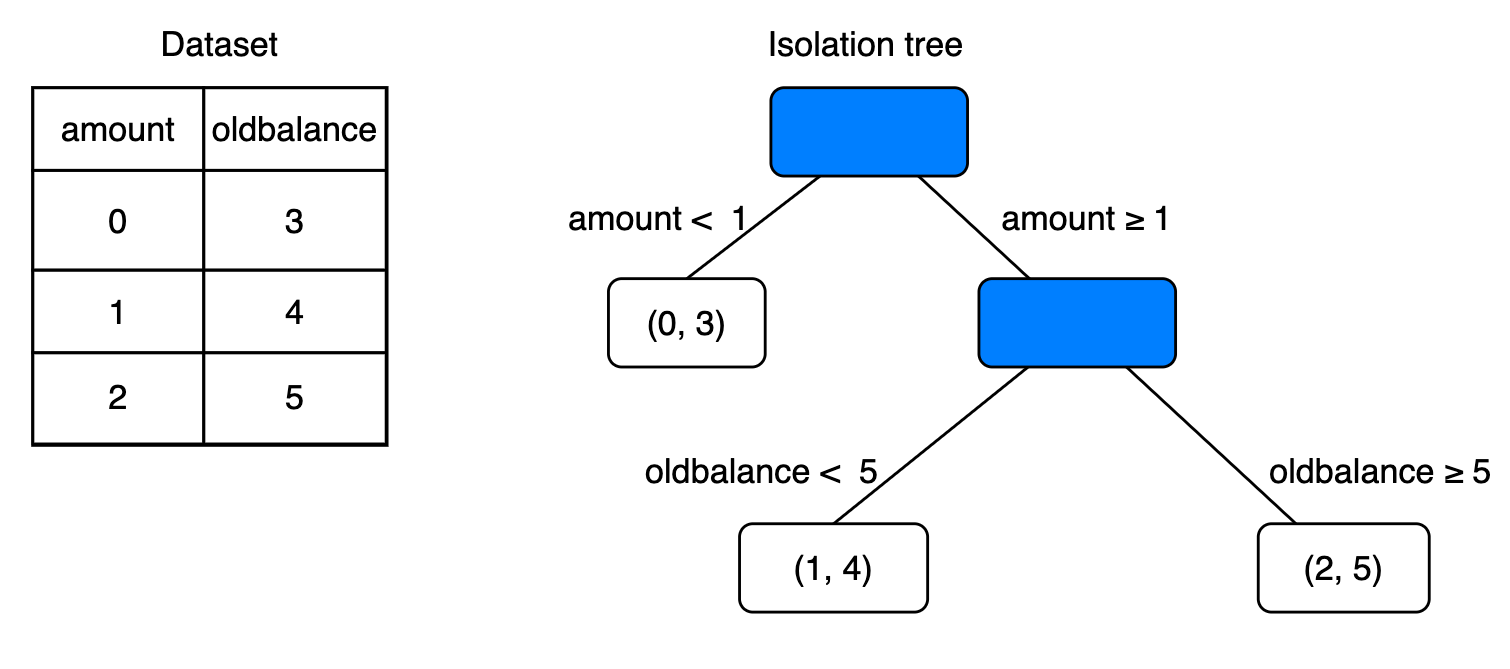
\includegraphics[width=\linewidth]{body/02_methodology/img/figure6.png}
  \caption{Illustration of the Isolation Forest algorithm.}
\end{figure}

We then need a metric to measure the degree of isolation of each data point. This metric is called the \textbf{anomaly score}. The anomaly score is calculated as follows:

\begin{equation}
    s(x, n) = 2^{-\frac{E(h(x))}{c(n)}}
\end{equation}

where 

\begin{itemize}
  \item $x$ is a data point.
  \item $n$ is the number of data points.
  \item $E(h(x))$ is the average value of $h(x)$.
  \item $h(x)$ is the path length of data point $x$.
  \newpage
  \item and $c(n)$ is the average path length of unsuccessful search in a binary tree, which is given by:
  \begin{equation}
    c(n)=\left\{
    \begin{array}{@{}ll@{}}
      2\ln(n-1) - \frac{2(n-1)}{n}, & \textrm{if } n>2 \\
      1, & \textrm{if } n=2 \\
      0, & otherwise
    \end{array}\right.
  \end{equation} 

where $H(i)$ is the harmonic number and is approximately equal to $\ln(i) + \mathrm{e}$.
\end{itemize}

This is the python code for calculating the anomaly score, the completed code can be found in the attached file:

\begin{lstlisting}[language=Python]
  def c(size):
      if size > 2:
          return 2 * (np.log(size-1)+0.5772156649) - 2*(size-1)/size
      if size == 2:
          return 1
      return 0
  
  def anomaly_score(X) -> np.ndarray:
      avg_length = self.path_length(X)
      scores = np.array([np.power(2, -l/c(sample_size))for l in avg_length])
      return scores
\end{lstlisting}
  

The anomaly score $\textbf{s(x, n)}$ is a value between 0 and 1. The closer the score is to 1, the more likely it is that the data point is an anomaly. The anomaly score is then used to determine whether a data point is an anomaly or not. If the score is greater than a predefined threshold, the data point is considered an anomaly. Otherwise, it is considered normal.
